\documentclass[titlepage,a4paper,12pt,AutoFakeBold]{article}
%\NeedsTeXFormat{LaTeX2e}[2005/12/01]
\usepackage{xeCJK}
\IfFontExistsTF{SimSun}{
	\setCJKmainfont{SimSun}
	\setCJKsansfont{SimSun}
	\setCJKmonofont{SimSun}
}{
	\IfFontExistsTF{Songti SC}{
		\setCJKmainfont{Songti SC}
		\setCJKsansfont{Songti SC}
		\setCJKmonofont{Songti SC}
	}{
		\setCJKmainfont{FandolSong-Regular}
		\setCJKsansfont{FandolHei-Regular}
		\setCJKmonofont{FandolFang-Regular}
	}
}
%\usepackage[margin=1in]{geometry}
\usepackage{geometry}
\geometry{a4paper,left=3.18cm,right=3.18cm,top=2.54cm,bottom=2.54cm}
\usepackage{braket}
\usepackage{graphicx}


\usepackage[hidelinks]{hyperref}
\hypersetup{
%linkbordercolor={1 1 1},
urlcolor=blue,
}
\usepackage{float}
\usepackage[bottom]{footmisc}

\usepackage{algorithm}
\usepackage[noend]{algpseudocode}
%\usepackage{longtable}
\usepackage{amsmath}
\usepackage{amssymb}
\usepackage{extarrows}
%\usepackage{tabularx}
%\usepackage{rotating}
\usepackage {indentfirst}
\usepackage{courier}
\setmonofont{lmmono10-regular.otf}
\setlength{\emergencystretch}{2em}
\usepackage[dvipsnames]{xcolor}
\usepackage{listings}
\usepackage[normalem]{ulem}


%\usepackage{xcolor}\lstset{}
\lstset{
	basicstyle={\sffamily\footnotesize},
	%	numbers=left,
	%	numberstyle=\tiny\color{gray},
	numbersep=5pt,
	breaklines=true,
	captionpos={T},
	frame={lines},
%%	rulecolor=,
	framerule=0.5pt,
	columns=flexible,
	tabsize=2,
	numbers=left,
%	backgroundcolor = \color{White},
	backgroundcolor={\color{yellow!3!white}}
%	language=Mathematica,
%	keywordstyle=\color{black}
}
\usepackage{enumitem}
% Keep each short code example together, including its closing bracket.
\usepackage{etoolbox}
\BeforeBeginEnvironment{lstlisting}{\par\noindent\begin{minipage}{\linewidth}}
\AfterEndEnvironment{lstlisting}{\end{minipage}\par}
%\allowdisplaybreaks[4]
%\usepackage{mathematica}
%\definecolor{darkred}{rgb}{0.5 0 0}
%\definecolor{darkgreen}{rgb}{0.5 .5 0}
%\definecolor{darkblue}{rgb}{0 0 .5}



%\usepackage{listings}
%\renewcommand{\lstlistingname}{Listing}


\renewcommand{\contentsname}{目录}
\renewcommand{\figurename}{图}
\newcommand\litem[1]{\item{ #1？\\}}
%\newcommand{\dollar}{\mbox{\textdollar}} \bfseries

\makeatletter

\makeatother






\begin{document}



\title{\textsf{MagneticTB}使用手册}
%\vtitle{利用群表示理论研究三维晶体中的演生粒子}
%\author{张泽英}
\author{张泽英}

\maketitle

%\newpage

\tableofcontents

\begin{quote}
\small
本手册介绍\textsf{MagneticTB} 2.0的常用功能。第一次使用时，可以先安装程序包，
再按第~\ref{gra}~节的石墨烯例子依次运行。
\end{quote}
\newpage

\section{功能简介}
\textsf{MagneticTB}是一款开源的软件包。
该软件包基于磁群的共表示理论开发，可以根据晶体对称性和局域轨道生成紧束缚模型。
构造模型时，需要给出晶格矢量、Wyckoff位置、磁化方向、对称操作和基函数。
有了这些输入，就可以求出对称性允许的Hamiltonian，再指定参数画出能带。
具体功能如下：
\begin{itemize}
\item 获取磁空间群、磁层群和磁杆群的对称操作；
\item 构造磁性与非磁性材料的紧束缚模型，包括非共线磁结构；
\item 构造不考虑自旋的模型，以及考虑自旋轨道耦合的双群模型；
\item 从参考格点的局域轨道出发，用诱导表示构造其他等价格点上的基函数；
\item 画晶体结构、磁矩、第一布里渊区和能带，并随参数大小动态显示能带；
\item 读写Wannier90格式文件，与能带拟合、能带表示计算等功能配合使用。
\end{itemize}

\section{安装、更新和卸载}
\subsection{安装与加载}
取得本地的\lstinline|.paclet|文件后，在Mathematica中运行：
\begin{lstlisting}[numbers=none]
PacletInstall["/absolute/path/MagneticTB-2.0.10.paclet"]
\end{lstlisting}
其中路径和文件名要换成实际文件。Windows用户也可以用正斜杠写路径，
例如\lstinline|"C:/Users/yourname/Downloads/MagneticTB-2.0.10.paclet"|。

安装后先保存正在编辑的Notebook，\textbf{完整退出并重新打开Mathematica}，
不只是重启内核。重新打开后，运行：
\begin{lstlisting}[numbers=none]
Needs["MagneticTB`"]
\end{lstlisting}
即可加载程序包。接下来仍需要用\lstinline|init|给出要研究的模型，
不能只运行加载命令就直接调用\lstinline|symham|。

\subsection{打开帮助文档}
在Mathematica的文档中心搜索\textsf{MagneticTB}，或直接运行：
\begin{lstlisting}[numbers=none]
SystemOpen["paclet:MagneticTB/guide/MagneticTB"]
\end{lstlisting}
即可打开图~\ref{fig:help-home}所示的帮助主页。
从“MagneticTB入门”开始，可以逐步运行安装、加载和第一个模型的例子；
继续向下浏览，可以按主题查找函数。
\begin{figure}[H]
\centering
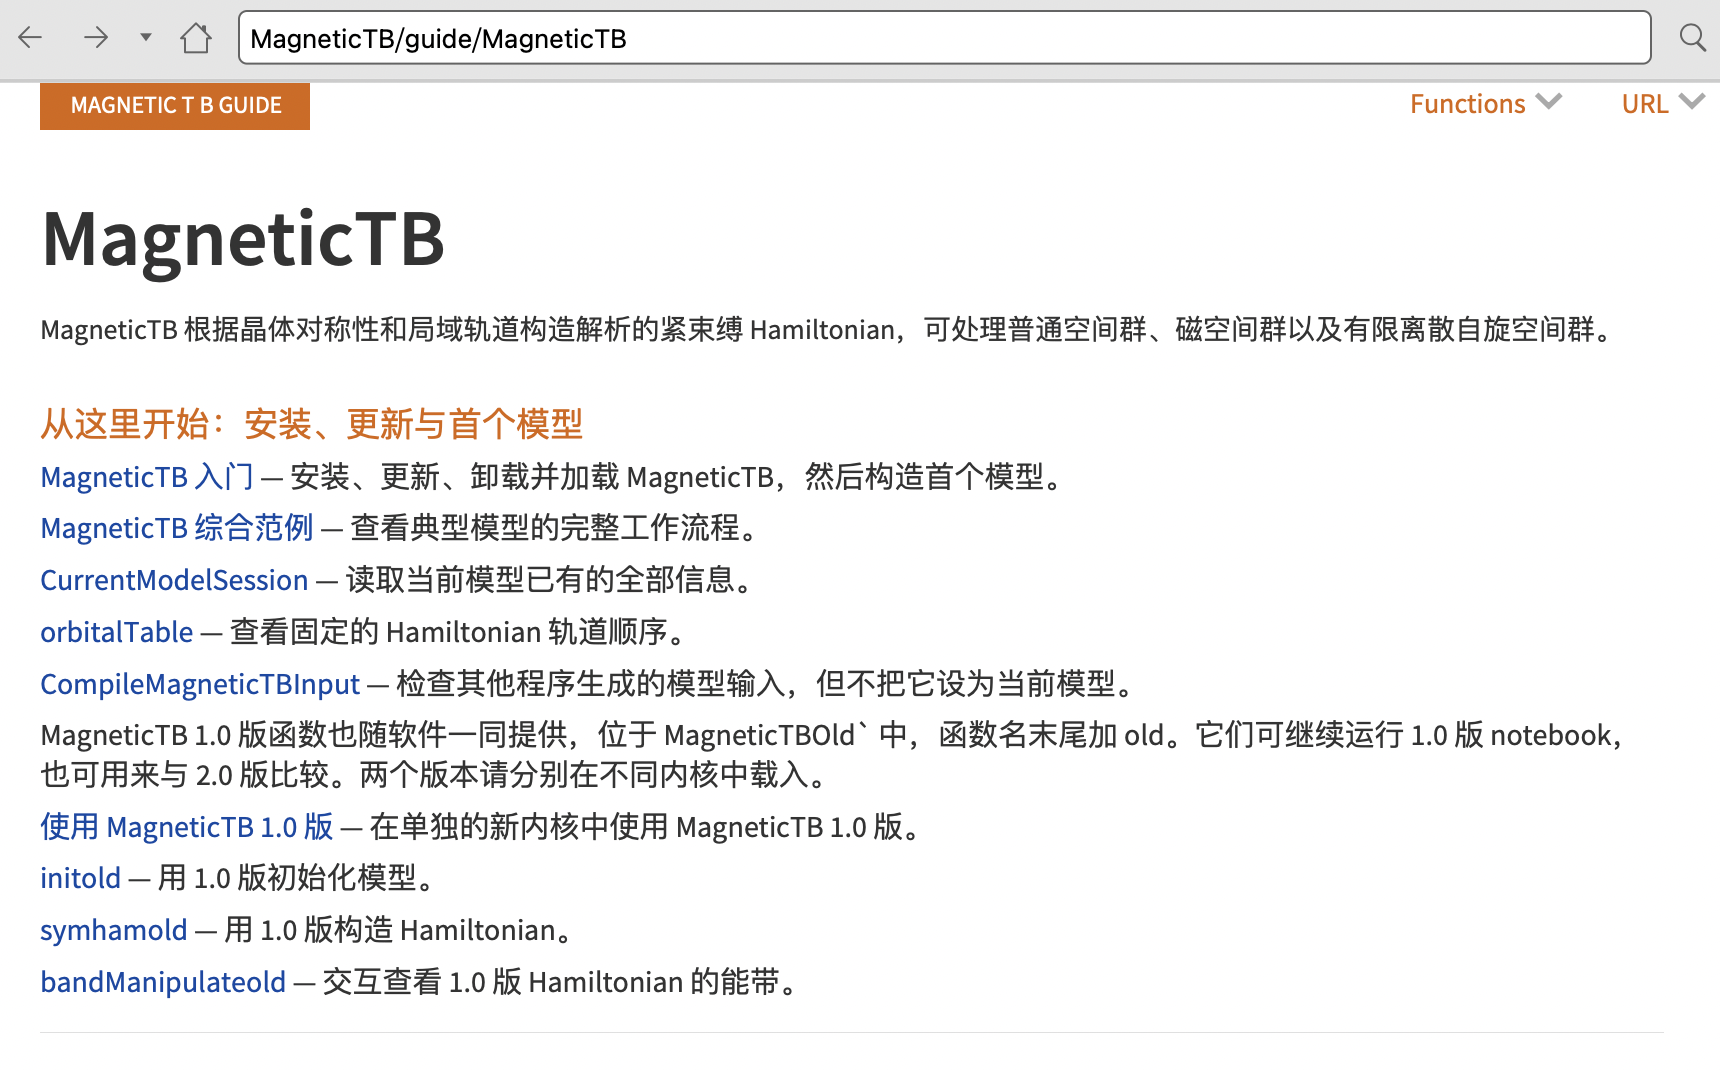
\includegraphics[width=\textwidth]{figures/manual-help-home.png}
\caption{Mathematica中的MagneticTB帮助主页。
点击蓝色文字可以进入相应的教程或函数页。}
\label{fig:help-home}
\end{figure}
例如，想直接查看初始化的用法，可以运行：
\begin{lstlisting}[numbers=none]
SystemOpen["paclet:MagneticTB/ref/init"]
\end{lstlisting}
本手册中的图是静态插图；\lstinline|bandManipulate|的滑块需要在Mathematica中操作。

\subsection{更新}
更新时，安装版本号更高的本地文件即可：
\begin{lstlisting}[numbers=none]
PacletInstall["/absolute/path/MagneticTB-<new-version>.paclet"]
\end{lstlisting}
然后保存工作，完整退出并重新打开Mathematica。运行
\lstinline|PacletFind["MagneticTB"]|可以查看已安装的版本。
目前不提供自动在线更新命令。

若提示\lstinline|PacletInstall::samevers|，说明这个版本已经安装。
确实要重新安装同一版本时，先卸载再安装：
\begin{lstlisting}[numbers=none]
PacletUninstall["MagneticTB"]
PacletInstall["/absolute/path/MagneticTB-2.0.10.paclet"]
\end{lstlisting}

\subsection{卸载}
不再使用时，运行：
\begin{lstlisting}[numbers=none]
PacletUninstall["MagneticTB"]
\end{lstlisting}
这会卸载程序包，不会删除用户自己保存的模型Notebook。
卸载后同样需要退出并重新打开Mathematica，以免继续使用已经载入内核的函数。

\section{使用方法}
\subsection{获取对称操作}
\textsf{MagneticTB}构造模型的主要流程由三个函数完成：
\lstinline|msgop|获取对称操作，\lstinline|init|设置模型，
\lstinline|symham|求出Hamiltonian。

对于非磁性材料，通常使用包含时间反演对称性的灰群。例如：
\begin{lstlisting}
Needs["MagneticTB`"];
sgop = msgop[gray[191]];
\end{lstlisting}
其中\lstinline|gray[191]|取得第191号空间群对应灰群的编码，
\lstinline|msgop|把编码转换为完整的对称操作列表。
程序同时打印磁群的BNS编号、符号和晶格矢量。
按BNS编号指定磁群时，例如$191.239$，写成：
\begin{lstlisting}[numbers=none]
msgop[bnsdict[{191, 239}]]
\end{lstlisting}
因此，\lstinline|gray|、\lstinline|bnsdict|一般和\lstinline|msgop|一起使用，
不需要记住程序内部的编码。

每个对称操作写成
\lstinline|{名称, 旋转矩阵, 平移矢量, "F"或"T"}|。
旋转和平移采用晶格基矢下的分数坐标；\lstinline|"T"|表示包含时间反演，
\lstinline|"F"|表示不包含时间反演。若换了一组晶格基矢，
对称操作也要变换到同一组基矢下，不能只修改晶格夹角。
磁层群和磁杆群采用相同的用法：
\begin{lstlisting}[numbers=none]
mlgop[graylayer[80]]
mrgop[grayrod[75]]
\end{lstlisting}
这里分别获取第80号层群和第75号杆群对应的灰群操作。

\subsection{初始化模型}
\label{sec:init}
有了对称操作，就可以使用\lstinline|init|设置晶格、原子位置和基函数。
以石墨烯为例，完整输入为：
\begin{lstlisting}
sgop = msgop[gray[191]];
init[
  lattice -> {
    {a, 0, 0}, {-a/2, Sqrt[3] a/2, 0}, {0, 0, c}
  },
  lattpar -> {a -> 1, c -> 3},
  wyckoffposition -> {{{1/3, 2/3, 0}, {0, 0, 0}}},
  symminformation -> sgop,
  basisFunctions -> {{"pz"}}
];
\end{lstlisting}
其中\lstinline|lattice|的三行分别是三个实空间晶格矢量；
\lstinline|lattpar|给出晶格矢量中参数的数值。
本例的面内夹角是$120^\circ$，层间距离取$c=3$。
\lstinline|symminformation|使用前面得到的完整对称操作列表。

\lstinline|wyckoffposition|给出不等价位置及其磁化方向，格式为
\[
\{\{\boldsymbol r_1,\boldsymbol m_1\},
  \{\boldsymbol r_2,\boldsymbol m_2\},\ldots\}.
\]
$\boldsymbol r_i$是分数坐标，$\boldsymbol m_i$是用晶格基矢表示的磁矩。
等价位置只需输入其中一个，程序会用对称操作生成其余位置。
上面的碳原子没有磁性，因此磁矩写为\lstinline|{0,0,0}|。

\lstinline|basisFunctions|与输入的不等价位置一一对应，
每个位置的基函数单独放在一个列表中。常用轨道的写法如下：
\begin{table}[H]
\centering
\begin{tabular}{cc|cc}
\hline
基函数 & 代码 & 基函数 & 代码\\
\hline
$s$ & \lstinline|"s"| & $p_x$ & \lstinline|"px"|\\
$p_y$ & \lstinline|"py"| & $p_z$ & \lstinline|"pz"|\\
$p_x+ip_y$ & \lstinline|"px+ipy"| & $p_x-ip_y$ & \lstinline|"px-ipy"|\\
$d_{z^2}$ & \lstinline|"dz2"| & $d_{xy}$ & \lstinline|"dxy"|\\
$d_{yz}$ & \lstinline|"dyz"| & $d_{xz}$ & \lstinline|"dxz"|\\
$d_{x^2-y^2}$ & \lstinline|"dx2-y2"| & &\\
\hline
\end{tabular}
\end{table}
考虑自旋时，在轨道名后加\lstinline|"up"|或\lstinline|"dn"|。
例如，碳原子的两个自旋态写成：
\begin{lstlisting}[numbers=none]
basisFunctions -> {{"pzup", "pzdn"}}
\end{lstlisting}
对于表中没有的轨道，也可以输入解析表达式。
例如$f_{xyz}$轨道写成：
\begin{lstlisting}[numbers=none]
basisFunctions -> {{x*y*z}}
\end{lstlisting}

初始化后，可以分别查看Hamiltonian的轨道顺序和晶体结构：
\begin{lstlisting}[numbers=none]
orbitalTable[]
showCrystalStructure[]
\end{lstlisting}
石墨烯会生成$(1/3,2/3,0)$和$(2/3,1/3,0)$两个碳原子，
每个原子有一个$p_z$轨道，因此Hamiltonian是一个$2\times2$矩阵。
如果要研究另一个模型，重新写完整的\lstinline|init[...]|即可。
MagneticTB不会沿用上一个模型。

\subsection{近邻与Hamiltonian}
\lstinline|symham[1]|给出在位能，\lstinline|symham[2]|给出最近邻跃迁，
\lstinline|symham[3]|给出第二近邻跃迁。每次调用只计算相应的一组距离，
不是自动把前面的项全部加起来。例如：
\begin{lstlisting}
ham = Sum[symham[i], {i, 3}];
MatrixForm[ham]
\end{lstlisting}
就得到包含在位能、最近邻和第二近邻的Hamiltonian。
程序给出的\lstinline|e1|、\lstinline|t1|、\lstinline|r1|等是独立参数，
它们的数值需要根据研究的问题指定，或用第一性原理能带拟合。

默认情况下，\lstinline|init|准备10组距离，其中第1组为在位项。
若要计算更远的近邻，在完整的\lstinline|init[...]|中加入
\lstinline|InitialBondShells -> 15|，再调用所需的\lstinline|symham[i]|。
普通的最近邻、第二近邻例子不需要写这个选项。

\lstinline|symham|默认构造厄米Hamiltonian。
若研究非厄米模型，将相应调用改为
\lstinline|symham[2, "Hermitian" -> False]|。
此时正向与反向的跃迁不再由厄米条件相互确定；
复能谱应根据研究目的分别画实部、虚部或复平面轨迹。

\subsection{画图模块}
运行\lstinline|init|后，可以直接画结构、第一布里渊区，并获取常用路径：
\begin{lstlisting}[numbers=none]
showCrystalStructure[]
showBrillouinZone[]
standardKPath[]
\end{lstlisting}
磁性模型的结构图还会显示磁矩箭头。三维图默认采用平行投影，
可以用Mathematica的\lstinline|Show|调整观察方向。

\lstinline|standardKPath|根据晶格度量选择内置的常用路径表，
不是空间群小群或不可约表示计算程序。
对于非标准基矢、中心化晶格或特殊路径，应核对点的坐标，
必要时自己输入所需路径。

得到Hamiltonian和路径后，画能带的用法为：
\begin{lstlisting}[numbers=none]
bandplot[path, n, ham, parameters]
bandManipulate[path, n, ham]
\end{lstlisting}
其中\lstinline|path|给出各段的端点及名称，\lstinline|n|控制每段的采样密度，
\lstinline|parameters|给出参数数值。
\lstinline|bandplot|画固定参数的能带，\lstinline|bandManipulate|用滑块调节参数。
若希望采用自动路径，可以写：
\begin{lstlisting}[numbers=none]
bandManipulate[standardKPath[], 80, ham]
\end{lstlisting}

路径中的点采用倒空间分数坐标，例如$K=(1/3,1/3,0)$。
默认Hamiltonian中的\lstinline|kx|、\lstinline|ky|、\lstinline|kz|则包含$2\pi$：
直接求$K$点的Hamiltonian时，应代入\lstinline|2 Pi {1/3,1/3,0}|。
画图函数会完成这个转换，不要再把路径乘一次$2\pi$。

\subsection{Wannier90接口}
已经求过\lstinline|symham[1]|到\lstinline|symham[3]|后，
可以把这三项写成Wannier90格式文件：
\begin{lstlisting}[numbers=none]
hop[3, parameters, "hrExport" -> "/absolute/path/wannier90_hr.dat"]
\end{lstlisting}
其中\lstinline|parameters|必须给出所有跃迁参数的数值。
这里直接导出已经求出的实空间跃迁，不需要对$H(\boldsymbol k)$作反傅里叶变换。
\lstinline|hop[ham, parameters]|形式仍用于从显式Bloch Hamiltonian提取跃迁；
若转换自己写的Hamiltonian，要核对轨道中心和相位约定。

读取文件并恢复Hamiltonian，可以写：
\begin{lstlisting}
hrData = readHR["/absolute/path/wannier90_hr.dat"];
buildBlochHamiltonian[hrData, {0, 0, 0}] // MatrixForm
\end{lstlisting}
第二行显示$\Gamma$点的Hamiltonian。改变其中的三分量分数坐标，
即可得到其他$\boldsymbol k$点的矩阵。文件中的轨道顺序就是矩阵的行列顺序。

\subsection{能带表示}
计算能带共表示需要另行安装\textsf{MSGCorep}及其所需的\textsf{SpaceGroupIrep}。
在新内核中先由用户显式加载依赖：
\begin{lstlisting}[numbers=none]
Needs["MSGCorep`"];
Needs["MagneticTB`"];
operations = getMSGElemFromMSGCorep[{164, 87}];
\end{lstlisting}
将得到的\lstinline|operations|按原顺序传给完整的\lstinline|init|，
并采用对应的晶格矢量。得到Hamiltonian后，使用
\lstinline|getTBBandCorep[BNSNo, ham, parameters, kset]|打印各个$\boldsymbol k$点的
能量、简并度和共表示名称。标量轨道走单值路线，
\lstinline|{"sup","sdn"}|等旋量基走双值路线。

这个接口只适用于\lstinline|getMSGElemFromMSGCorep|产生的操作，
不能换成\lstinline|msgop|或其他来源的操作列表。
完整例子见帮助主页中的“能带共表示”教程。
程序不会替用户加载依赖，也不会用内部近似结果代替外部计算。

\section{例子}
\subsection{石墨烯}
\label{gra}
要生成石墨烯费米面附近的紧束缚模型，只需知道两个碳原子位于第191号空间群的
$2c$ Wyckoff位置，以及费米面附近的电子态由碳原子的$p_z$轨道构成。
具体代码如下：
\begin{lstlisting}
Needs["MagneticTB`"];
sgop = msgop[gray[191]];
init[
  lattice -> {
    {a, 0, 0}, {-a/2, Sqrt[3] a/2, 0}, {0, 0, c}
  },
  lattpar -> {a -> 1, c -> 3},
  wyckoffposition -> {{{1/3, 2/3, 0}, {0, 0, 0}}},
  symminformation -> sgop,
  basisFunctions -> {{"pz"}}
];
\end{lstlisting}
其中第2行获取第191号灰群的全部对称操作。
\lstinline|wyckoffposition|只写一个碳原子，另一个等价碳原子由程序生成。
为看清平面内的排列，可以画$3\times3$个原胞的俯视图：
\begin{lstlisting}
Show[
  showCrystalStructure[
    "CellRange" -> {{0, 2}, {0, 2}, {0, 0}}, ImageSize -> 440
  ],
  ViewPoint -> {0, 0, 3}, ViewVertical -> {0, 1, 0}
]
\end{lstlisting}
\lstinline|"CellRange"|只改变画出的晶胞范围，不改变Hamiltonian的大小。
图中的球是碳原子，灰线是晶胞边界，不是跃迁键。

面内的能带取$\Gamma$--$M$--$K$--$\Gamma$路径，可以从六方路径中取前三段：
\begin{lstlisting}
path = Take[standardKPath[], 3];
showBrillouinZone["KPath" -> path, ImageSize -> 440]
\end{lstlisting}
这三段的端点依次为
$\Gamma=(0,0,0)$、$M=(1/2,0,0)$、$K=(1/3,1/3,0)$和$\Gamma$。
布里渊区图中的彩色线就是下面画能带时使用的路径。
\begin{figure}[H]
\centering
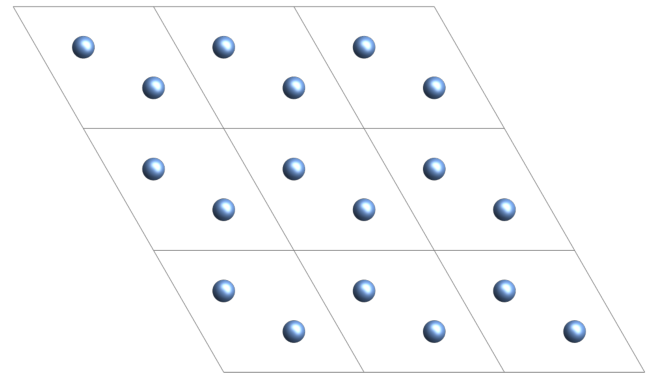
\includegraphics[width=.48\textwidth]{figures/manual-graphene-structure.pdf}
\hfill
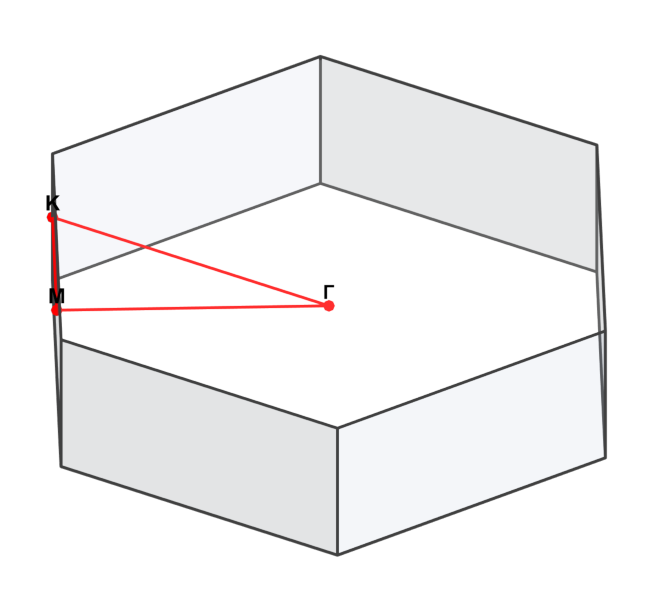
\includegraphics[width=.48\textwidth]{figures/manual-graphene-bz.pdf}
\caption{石墨烯的原子排列（左）和第一布里渊区（右）。
左图为18个碳原子的俯视图；右图中的路径位于$k_z=0$平面。}
\label{fig:graphene-structure}
\end{figure}

检查结构无误后，生成包含在位能、最近邻和第二近邻跃迁的Hamiltonian：
\begin{lstlisting}
ham = Sum[symham[i], {i, 3}];
MatrixForm[ham]
\end{lstlisting}
矩阵的两行分别对应两个碳原子的$p_z$轨道。对角项含在位能和同一子晶格间的
第二近邻跃迁，非对角项来自两个子晶格间的最近邻跃迁。
\lstinline|e1|是共同的在位能，\lstinline|t1|和\lstinline|r1|分别控制最近邻与
第二近邻跃迁。

把指数项合并后，这个矩阵可以写为
\[
H(\boldsymbol k)=\begin{pmatrix}d(\boldsymbol k)&t_1 f(\boldsymbol k)\\
t_1 f(\boldsymbol k)^*&d(\boldsymbol k)\end{pmatrix},
\]
其中
\begin{align*}
d(\boldsymbol k)&=e_1+2r_1[\cos k_x+\cos k_y+\cos(k_x+k_y)],\\
f(\boldsymbol k)&=e^{i(k_x-k_y)/3}(1+e^{-ik_x}+e^{ik_y}).
\end{align*}
三个指数项来自三条最近邻键。在$K$点它们相互抵消，因而两条能带相交。

给参数赋值后，一行命令就可以画出能带：
\begin{lstlisting}
parameters = {e1 -> 0.05, t1 -> 0.5, r1 -> 0.02};
bandplot[path, 80, ham, parameters, ImageSize -> 440, FontSize -> 16]
\end{lstlisting}
\begin{figure}[H]
\centering
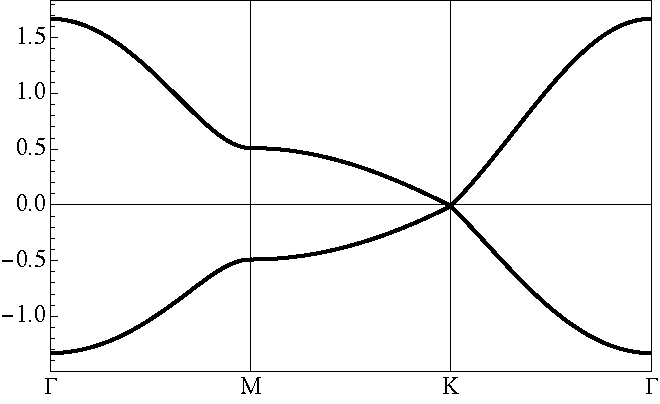
\includegraphics[width=.72\textwidth]{figures/manual-graphene-band.pdf}
\caption{石墨烯的两条$p_z$能带。参数取$e_1=0.05$、$t_1=0.5$、$r_1=0.02$。
两条能带在$K$点相交；第二近邻跃迁改变能带形状，但没有打开这个交叉点的带隙。}
\label{fig:graphene-band}
\end{figure}
图中的能量单位由参数单位决定；若参数用eV输入，纵轴就是eV。
想直接观察参数对能带的影响，可以运行：
\begin{lstlisting}[numbers=none]
bandManipulate[path, 80, ham]
\end{lstlisting}
在Notebook中调节\lstinline|t1|和\lstinline|r1|的滑块即可看到变化。

这个模型也可以直接导出：
\begin{lstlisting}[numbers=none]
hop[3, parameters, "hrExport" -> "/absolute/path/graphene_hr.dat"]
\end{lstlisting}
不需要把完整的跃迁表打印到屏幕上。若要查看某个近邻对应的原子和距离，
再单独使用\lstinline|showbonds[2]|或\lstinline|showbonds[3]|即可。

\subsubsection{考虑自旋轨道耦合}
若要考虑自旋轨道耦合，把每个碳原子的$p_z$轨道换成
$p_z\uparrow$和$p_z\downarrow$两个基函数。完整输入为：
\begin{lstlisting}
init[
  lattice -> {
    {a, 0, 0}, {-a/2, Sqrt[3] a/2, 0}, {0, 0, c}
  },
  lattpar -> {a -> 1, c -> 3},
  wyckoffposition -> {{{1/3, 2/3, 0}, {0, 0, 0}}},
  symminformation -> sgop,
  basisFunctions -> {{"pzup", "pzdn"}}
];
hamsoc = Sum[symham[i], {i, 3}];
MatrixForm[hamsoc]
\end{lstlisting}
此时矩阵有四行，依次对应第一个碳原子的两个自旋态和第二个碳原子的两个自旋态。
晶格、位置和空间群都没有改变，但程序会按旋量基生成双群表示。
因此，不能只把前面的两带Hamiltonian简单复制两份来代替SOC模型。
在这个四带模型中，\lstinline|r1|控制自旋相关的第二近邻跃迁，
\lstinline|r2|控制自旋无关的第二近邻跃迁。
注意：这里的\lstinline|r1|已不是前面两带模型中同名参数的含义。
分别把SOC参数取为0和0.05，可以直接比较能带：
\begin{lstlisting}
bandplot[
  path, 80, hamsoc, {e1 -> 0.05, t1 -> 0.5, r1 -> 0, r2 -> 0.02},
  ImageSize -> 440, FontSize -> 16
]
bandplot[
  path, 80, hamsoc, {e1 -> 0.05, t1 -> 0.5, r1 -> 0.05, r2 -> 0.02},
  ImageSize -> 440, FontSize -> 16
]
\end{lstlisting}
\begin{figure}[H]
\centering
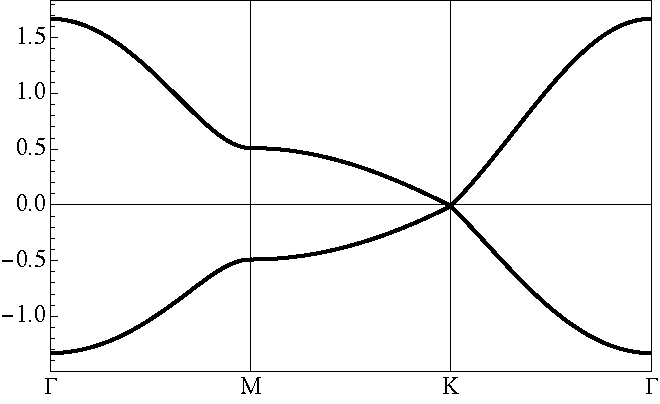
\includegraphics[width=.48\textwidth]{figures/manual-graphene-soc-off.pdf}
\hfill
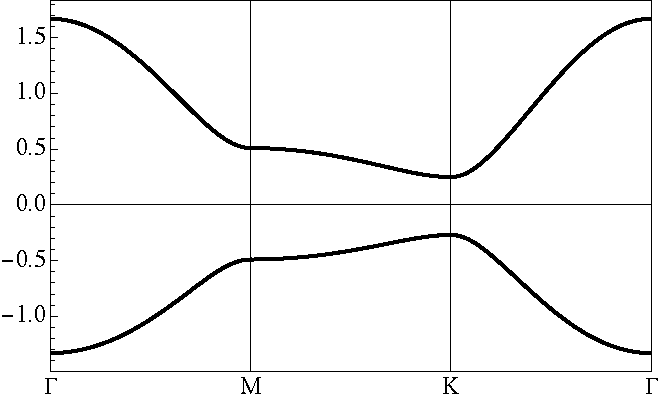
\includegraphics[width=.48\textwidth]{figures/manual-graphene-soc-on.pdf}
\caption{同一个四带石墨烯模型，SOC参数为0（左）和0.05（右）。
右图在$K$点打开带隙；每条可见能带仍为二重简并。}
\label{fig:graphene-soc}
\end{figure}

\subsection{立方晶格中的诱导表示}
\label{sec:induced}
有些模型中，只想保留每个原子上沿局域轴方向的一个$p$轨道。
但立方群中的旋转会把$p_x$变成$p_y$或$p_z$，如果要求每个原子上都使用同一套
固定的局域基，就必须同时输入$p_x,p_y,p_z$。
诱导模式可以从参考原子上的一个$p_x$出发，由对称操作确定其他等价原子上的轨道。

例如，第221号空间群中，从$(1/2,0,0)$出发会得到三个等价位置。
参考原子只保留$p_x$，输入为：
\begin{lstlisting}
Needs["MagneticTB`"];
init[
  lattice -> {{a, 0, 0}, {0, a, 0}, {0, 0, a}},
  lattpar -> {a -> 1},
  wyckoffposition -> {{{1/2, 0, 0}, {0, 0, 0}}},
  symminformation -> msgop[gray[221]],
  basisFunctions -> {{"px"}},
  RepresentationMode -> "Induced"
];
orbitalTable[]
\end{lstlisting}
其中\lstinline|RepresentationMode -> "Induced"|表示使用诱导模式。
轨道表的三行依次是$(1/2,0,0)$处的$p_x$、$(0,0,1/2)$处的$p_z$和
$(0,1/2,0)$处的$p_y$。这里没有在三个原子上都放置同一个$p_x$，
而是由立方群的旋转确定了另外两个原子上的轨道方向。

画出结构和最近邻模型的能带：
\begin{lstlisting}
showCrystalStructure[
  "CellRange" -> {{0, 1}, {0, 1}, {0, 1}}, ImageSize -> 440
]
hamCubic = Simplify[ComplexExpand[symham[1] + symham[2]]];
hamCubic // MatrixForm
pathCubic = standardKPath[];
bandplot[
  pathCubic, 60, hamCubic, {e1 -> 0, t1 -> -1},
  ImageSize -> 440, FontSize -> 16
]
\end{lstlisting}
\begin{figure}[H]
\centering
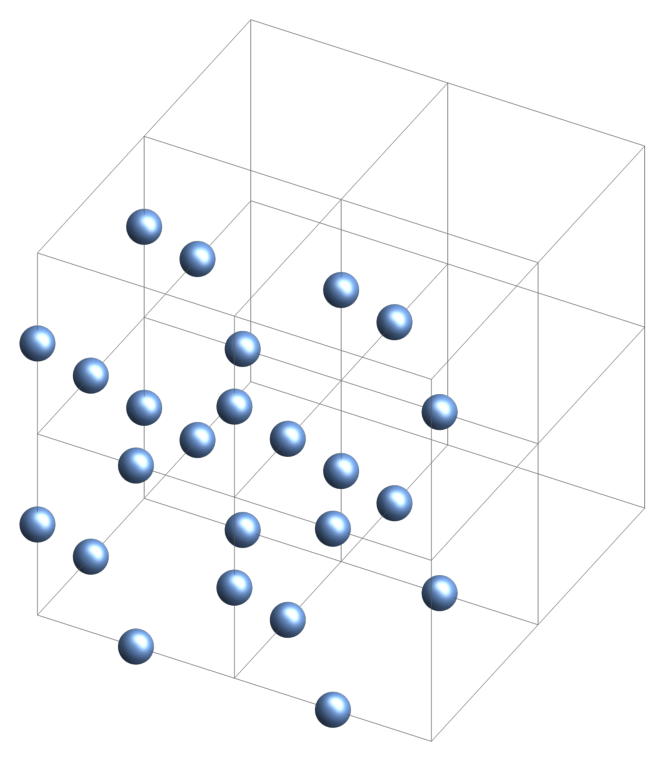
\includegraphics[width=.46\textwidth]{figures/manual-cubic-structure.pdf}
\hfill
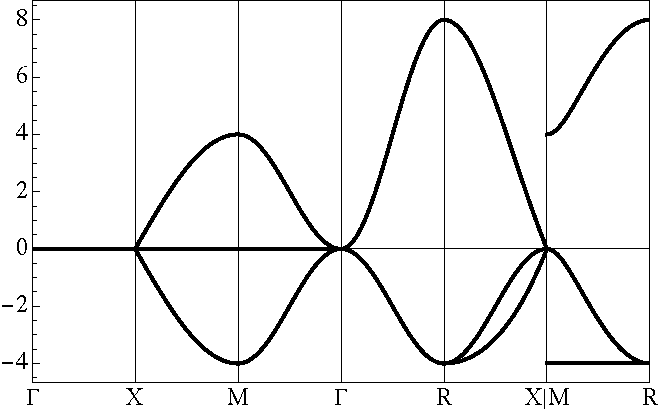
\includegraphics[width=.50\textwidth]{figures/manual-cubic-band.pdf}
\caption{立方晶格诱导模型的等价原子（左）和三条能带（右）。
每个原子只保留一个由参考$p_x$搬运得到的轨道。结构图只显示原子位置，
不显示$p$轨道波瓣。}
\label{fig:cubic-induced}
\end{figure}
按上述轨道顺序，矩阵可以写成
\[
H(\boldsymbol k)=e_1 I_3-4t_1
\begin{pmatrix}
0&s_xs_z&s_xs_y\\s_xs_z&0&s_ys_z\\s_xs_y&s_ys_z&0
\end{pmatrix},\qquad s_i=\sin(k_i/2).
\]
因此，沿$\Gamma$--$X$方向三条能带重合在$e_1$处；
沿$X$--$M$方向，两条能带向上下分开，另一条保持在$e_1$。
图中的$X|M$表示路径从$X$跳到$M$后继续画下一段，不把这两个点连起来。

若改用默认的\lstinline|"DirectProduct"|模式，应在同一个完整初始化中把最后两项改为：
\begin{lstlisting}[numbers=none]
basisFunctions -> {{"px", "py", "pz"}},
RepresentationMode -> "DirectProduct"
\end{lstlisting}
这时三个原子各有三个轨道，得到的是九带模型。
它和上面的三带模型不是同一组基函数，不能要求两者的整套能带完全相同。
诱导模式的作用是让用户只输入参考位置真正需要的局域态，
而不是自动删去一个九带模型中的任意六条带。

如果局域表示矩阵已经由其他程序给出，可以使用\lstinline|initfromrep|；
它接收表示矩阵而不是轨道字符串。这个入口要求完整且顺序固定的群，
不接受\lstinline|GenerateSymmetryGroup|。一般的轨道建模不需要使用它。

\subsection{非共线磁性Kagome模型}
\label{sec:kagome}
下面考虑三个面内磁矩相互夹角为$120^\circ$的Kagome模型。
三个原子的磁矩之和为0，但每个原子都有非零磁矩，不能把它当作非磁性模型。
采用磁空间群$191.239$，在参考位置上给出一个局域旋量：
\begin{lstlisting}
Needs["MagneticTB`"];
init[
  lattice -> {
    {a, 0, 0}, {-a/2, Sqrt[3] a/2, 0}, {0, 0, c}
  },
  lattpar -> {a -> 1, c -> 4},
  wyckoffposition -> {{{1/2, 0, 0}, {1, 0, 0}}},
  symminformation -> msgop[typeIII[{191, 239}]],
  basisFunctions -> {{{1, -1}/Sqrt[2]}},
  RepresentationMode -> "Induced"
];
\end{lstlisting}
其中\lstinline|typeIII[{191,239}]|按BNS编号指定这个第三类磁空间群。
\lstinline|{1,-1}/Sqrt[2]|的两个分量写在自旋$\uparrow,\downarrow$基下，
但它们共同构成\textbf{一个}局域态，不是两个独立基函数。
诱导模式把这个态搬运到另外两个等价格点，因此这个模型有三条能带，
而不是完整的六带自旋模型。

程序生成的位置依次为$(1/2,0,0)$、$(0,1/2,0)$和$(1/2,1/2,0)$。
对应磁矩在晶格基矢下为$(1,0,0)$、$(0,1,0)$和$(-1,-1,0)$。
由于面内基矢夹角为$120^\circ$，这三个磁矩在笛卡尔坐标下等长且互成$120^\circ$。

\subsubsection{看磁结构}
先画$2\times2$个原胞，再从上方看$3\times3$个原胞：
\begin{lstlisting}
showCrystalStructure[
  "CellRange" -> {{0, 1}, {0, 1}, {0, 0}},
  "MomentScale" -> 0.3, ImageSize -> 400
]
Show[
  showCrystalStructure[
    "CellRange" -> {{0, 2}, {0, 2}, {0, 0}},
    "MomentScale" -> 0.3, ImageSize -> 400
  ],
  ViewPoint -> {0, 0, 3}, ViewVertical -> {0, 1, 0}
]
\end{lstlisting}
\begin{figure}[H]
\centering
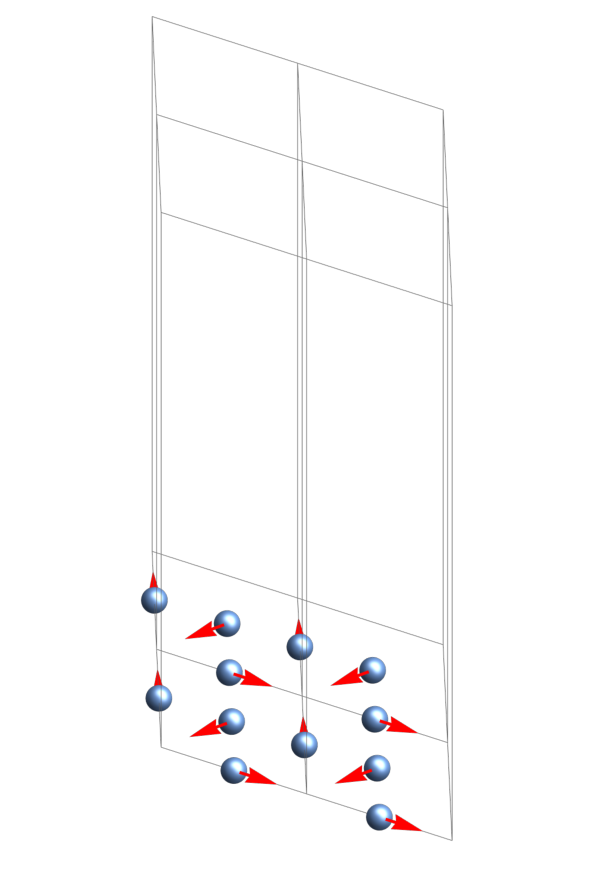
\includegraphics[height=.24\textheight]{figures/manual-kagome-structure.pdf}
\hfill
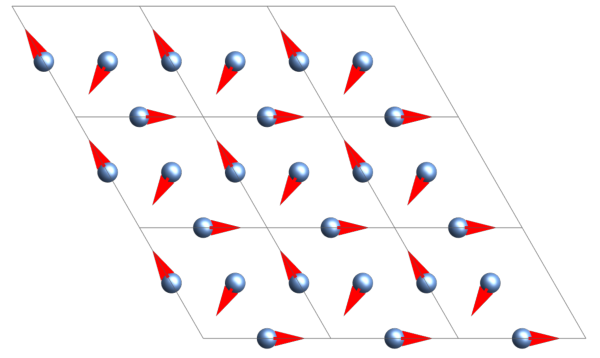
\includegraphics[width=.65\textwidth]{figures/manual-kagome-top.pdf}
\caption{非共线Kagome磁结构的斜视图（左）和俯视图（右）。
红色箭头由初始化中的磁矩直接生成；右图中可以看到三个磁矩方向周期性重复。}
\label{fig:kagome}
\end{figure}
\lstinline|"MomentScale"|只调节箭头的显示长度，不改变模型中的磁矩。
图中的灰线仍是晶胞边界，不是跃迁路径。

\subsubsection{看Hamiltonian和能带}
这个例子只考虑在位能和最近邻跃迁：
\begin{lstlisting}
kagomeHamiltonian = Simplify[ComplexExpand[symham[1] + symham[2]]];
kagomeHamiltonian // MatrixForm
\end{lstlisting}
其中\lstinline|ComplexExpand|和\lstinline|Simplify|把实动量下成对的指数函数写成余弦，
不改变模型。矩阵为
\[
H(\boldsymbol k)=
\begin{pmatrix}
 e_1 & 2t_1\cos\frac{k_x+k_y}{2} & 2t_1\cos\frac{k_y}{2}\\
 2t_1\cos\frac{k_x+k_y}{2} & e_1 & -2t_1\cos\frac{k_x}{2}\\
 2t_1\cos\frac{k_y}{2} & -2t_1\cos\frac{k_x}{2} & e_1
\end{pmatrix}.
\]
三个对角元相同，说明三个等价格点有共同的在位能。
非对角元中的相对负号由当前诱导旋量基生成，不能为了使矩阵看起来整齐而把它删去。

取$k_z=0$平面的$\Gamma$--$M$--$K$--$\Gamma$路径，直接画出布里渊区和能带：
\begin{lstlisting}
planePath = Take[standardKPath[], 3];
showBrillouinZone["KPath" -> planePath, ImageSize -> 400]
bandplot[
  planePath, 60, kagomeHamiltonian, {e1 -> 0, t1 -> -1},
  ImageSize -> 400, FontSize -> 16
]
\end{lstlisting}
\begin{figure}[H]
\centering
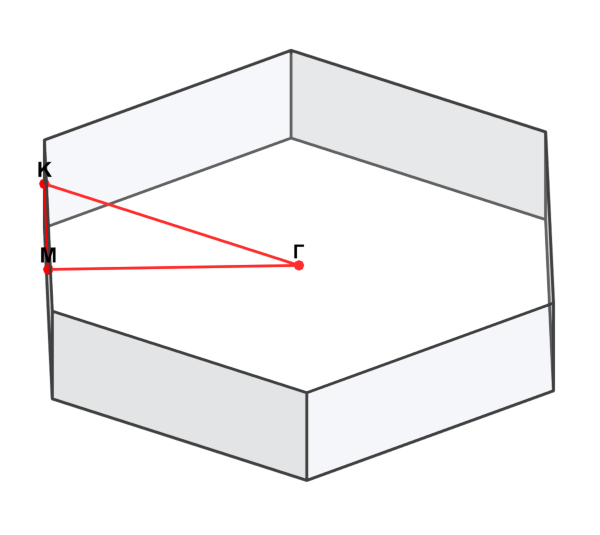
\includegraphics[width=.46\textwidth]{figures/manual-kagome-bz.pdf}
\hfill
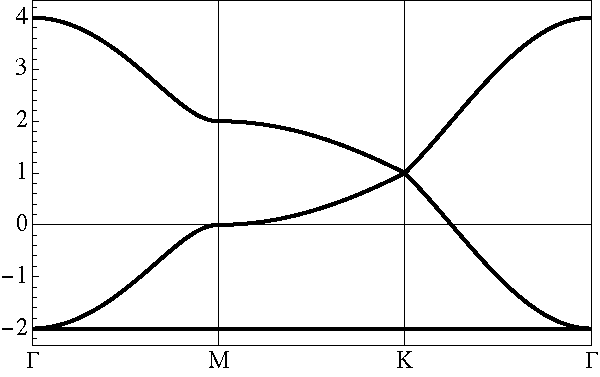
\includegraphics[width=.50\textwidth]{figures/manual-kagome-band.pdf}
\caption{同一个Kagome模型的面内路径（左）和能带（右）。
平带位于$E=-2$，两条色散带在$K$点的$E=1$处相交。}
\label{fig:kagome-band}
\end{figure}
在$\Gamma$点，平带与下方的色散带相接。这两组近邻没有层间跃迁，
所以Hamiltonian不含$k_z$。
这里给出的是一个理想磁性Kagome模型，参数用于说明对称性允许的能带，
不是某个具体材料的拟合参数。

\section{常见问题}
\begin{enumerate}[style=nextline]
\setlength\itemsep{1.2em}
\litem{安装后找不到帮助页怎么办}
回答：先运行\lstinline|PacletFind["MagneticTB"]|确认已经安装，
再保存工作，完整退出并重新打开Mathematica。
随后运行\lstinline|SystemOpen["paclet:MagneticTB/guide/MagneticTB"]|。
只重启内核可能仍会看到前端中已经打开的旧帮助页。

\litem{为什么只输入晶格常数，init不能生成模型}
回答：晶格常数只确定几何尺度，还没有告诉程序原子在哪里、满足什么对称性、
使用哪些轨道。应像第~\ref{sec:init}~节一样给出完整的五项模型输入，
不能把\lstinline|init[lattice -> ...]|当作一个完整模型。

\litem{从msgop得到的操作还要补全群吗}
回答：不需要。\lstinline|msgop|已经给出完整操作，
\lstinline|GenerateSymmetryGroup|的默认值也是\lstinline|False|。
只有自己仅输入生成元时，才在完整的\lstinline|init|中加入
\lstinline|GenerateSymmetryGroup -> True|。

\litem{为什么bandManipulate刚打开时能带全是水平线}
回答：滑块初值是0。在位能和跃迁全部为0时，Hamiltonian就是零矩阵。
把跃迁参数调离0，或用一组明确的参数调用\lstinline|bandplot|，
就可以看到模型的色散。

\litem{改变晶格基矢后，为什么Hamiltonian的表达式不同}
回答：动量坐标、原子分数坐标和对称操作都依赖所选的基矢。
例如六方晶格的面内夹角取$120^\circ$或$60^\circ$时，同一个物理模型会写成不同形式。
比较两个结果前，要先把晶格、位置、对称操作和动量路径转换到同一约定，
不能只比较参数名称或某个矩阵元。

\litem{只输入一个px，什么时候可以使用诱导模式}
回答：参考位置上的局域态必须在该位置的位点对称群作用下封闭。
第~\ref{sec:induced}~节的立方例子满足这个条件，因此可以从一个$p_x$出发。
不是任意位置、任意轨道都能只留一个分量；若位点对称操作把$p_x$变到另一个独立态，
就还需要把那个态加入参考基函数。

\litem{考虑自旋但不考虑SOC，能否直接删掉几个参数}
回答：不能仅凭参数名称判断。\textsf{MagneticTB}支持把空间作用和自旋作用分别给出，
也支持通过显式表示入口加入一个内部连续自旋旋转$C_\infty$。
无SOC模型应使用与磁结构相符的自旋对称性约束；完整的构造方法见帮助主页中的
“连续自旋对称性”教程，而不是把含SOC矩阵中的任意几项设为0。

\litem{还想计算模型的其他物性怎么办}
回答：可以继续使用程序包中的相应物性函数，也可以通过\lstinline|hop|导出
Wannier90格式文件，再交给其他软件计算。
不同函数对坐标和轨道中心的约定可能不同，使用时应先看对应帮助页，
不要把手写的动量函数与默认$H(\boldsymbol k)$的坐标约定混用。

\litem{如何使用1.0版}
回答：在新的内核中运行\lstinline|Needs["MagneticTBOld`"]|，
再调用\lstinline|initold|、\lstinline|symhamold|等对应函数。
1.0版与2.0版请分别在两个内核中加载。
具体输入见帮助主页中的“使用1.0版”教程。

\litem{哪里可以找到更多例子}
回答：安装paclet后，在帮助主页打开“MagneticTB综合范例”“晶体结构与k路径”
或能带拟合等教程。函数页还给出了相应选项的调用方法，
可以把例子中的参数改成自己的模型参数。

\litem{如何反馈问题}
回答：可以加入QQ群625192239，或在
\url{https://github.com/zhangzeyingvv/MagneticTB/issues}提问，
也可以发邮件到\href{mailto:zhangzeyingvv@gmail.com}{zhangzeyingvv@gmail.com}。
最好同时提供所用版本、完整输入和错误消息，便于重复问题。
\begin{figure}[H]
\centering

\includegraphics[width=.23\textwidth]{figures/QQ.jpg}
\end{figure}

\litem{如何引用MagneticTB}
回答：使用本程序包开展研究时，请引用：
Zeying Zhang, Zhi-Ming Yu, Gui-Bin Liu, Yugui Yao,
\textit{MagneticTB: A package for tight-binding model of magnetic and non-magnetic materials},
Computer Physics Communications \textbf{270}, 108153 (2022).
DOI: \href{https://doi.org/10.1016/j.cpc.2021.108153}{10.1016/j.cpc.2021.108153}。
\begin{lstlisting}[numbers=none,language=TeX]
@article{ZHANG2022108153,
  title = {MagneticTB: A package for tight-binding model
    of magnetic and non-magnetic materials},
  author = {Zhang, Zeying and Yu, Zhi-Ming and
    Liu, Gui-Bin and Yao, Yugui},
  journal = {Computer Physics Communications},
  volume = {270},
  pages = {108153},
  year = {2022},
  doi = {10.1016/j.cpc.2021.108153}
}
\end{lstlisting}
\end{enumerate}
\end{document}
